\subsection{Targeted Attacks and Null-Model Comparison}
\label{sec:targeted-attacks}

Random-failure experiments treat all nodes as equally likely to fail. However, nodes in a knowledge graph can differ substantially in their structural importance. A node connected to many other entities may act as a hub, while another node may connect otherwise weakly linked regions of the graph. We therefore ask how vulnerable the PrimeKG network is when structurally important nodes are deliberately removed first. We compare random node removal with two targeted strategies based on degree and betweenness centrality on the same 5,000-node PrimeKG subgraph.

\subsubsection{Centrality-Based Attack Strategies}
For a node $v$, its degree is
\begin{equation}
    k_v = \deg(v),
\end{equation}
which is the number of nodes directly connected to $v$. Nodes with high degree therefore act as local hubs with many direct connections. A degree-based attack removes nodes in decreasing order of degree.

Betweenness centrality instead measures how frequently a node lies on shortest paths between other nodes. For node $v$,
\begin{equation}
C_B(v)=\sum_{s\neq v\neq t}\frac{\sigma_{st}(v)}{\sigma_{st}},
\end{equation}
where $\sigma_{st}$ is the number of shortest paths between $s$ and $t$, and $\sigma_{st}(v)$ is the number of those paths that pass through $v$. Degree therefore emphasizes local connectivity, whereas betweenness emphasizes bridge or bottleneck roles.

For both targeted strategies, centrality scores are computed once on the intact graph and the resulting rankings are kept fixed throughout the experiment. The attack sequence is therefore a fixed original ranking rather than an adaptive strategy that recomputes centrality after every removal.

We quantify structural robustness using the giant connected component (GCC) fraction
\begin{equation}
S(f)=\frac{|\mathrm{GCC}(f)|}{N_0},
\end{equation}
where $f$ is the fraction of nodes removed, $|\mathrm{GCC}(f)|$ is the number of surviving nodes in the largest connected component, and $N_0$ is the original number of nodes. Because the denominator is fixed at the original graph size, directly removed nodes also count as lost.

\subsubsection{Robustness under Targeted Node Removal}
Figure~\ref{fig:ws2-attacks} compares random node failure with degree- and betweenness-based attacks. Targeted attacks consistently leave a smaller giant component than random removal. At $f=0.20$, random failure retains approximately 79.7\% of the original graph in the GCC, whereas degree and betweenness attacks retain approximately 69.0\% and 68.6\%, respectively. At $f=0.50$, the difference is substantially larger: $S_{\mathrm{random}}\approx0.493$, $S_{\mathrm{degree}}\approx0.232$, and $S_{\mathrm{betweenness}}\approx0.206$.

\begin{figure}[H]
    \centering
    % Repository path expected: figures/ws2_attack_curves_primekg_5000_bfs_v1.png
    \IfFileExists{../figures/ws2_attack_curves_primekg_5000_bfs_v1.png}{%
      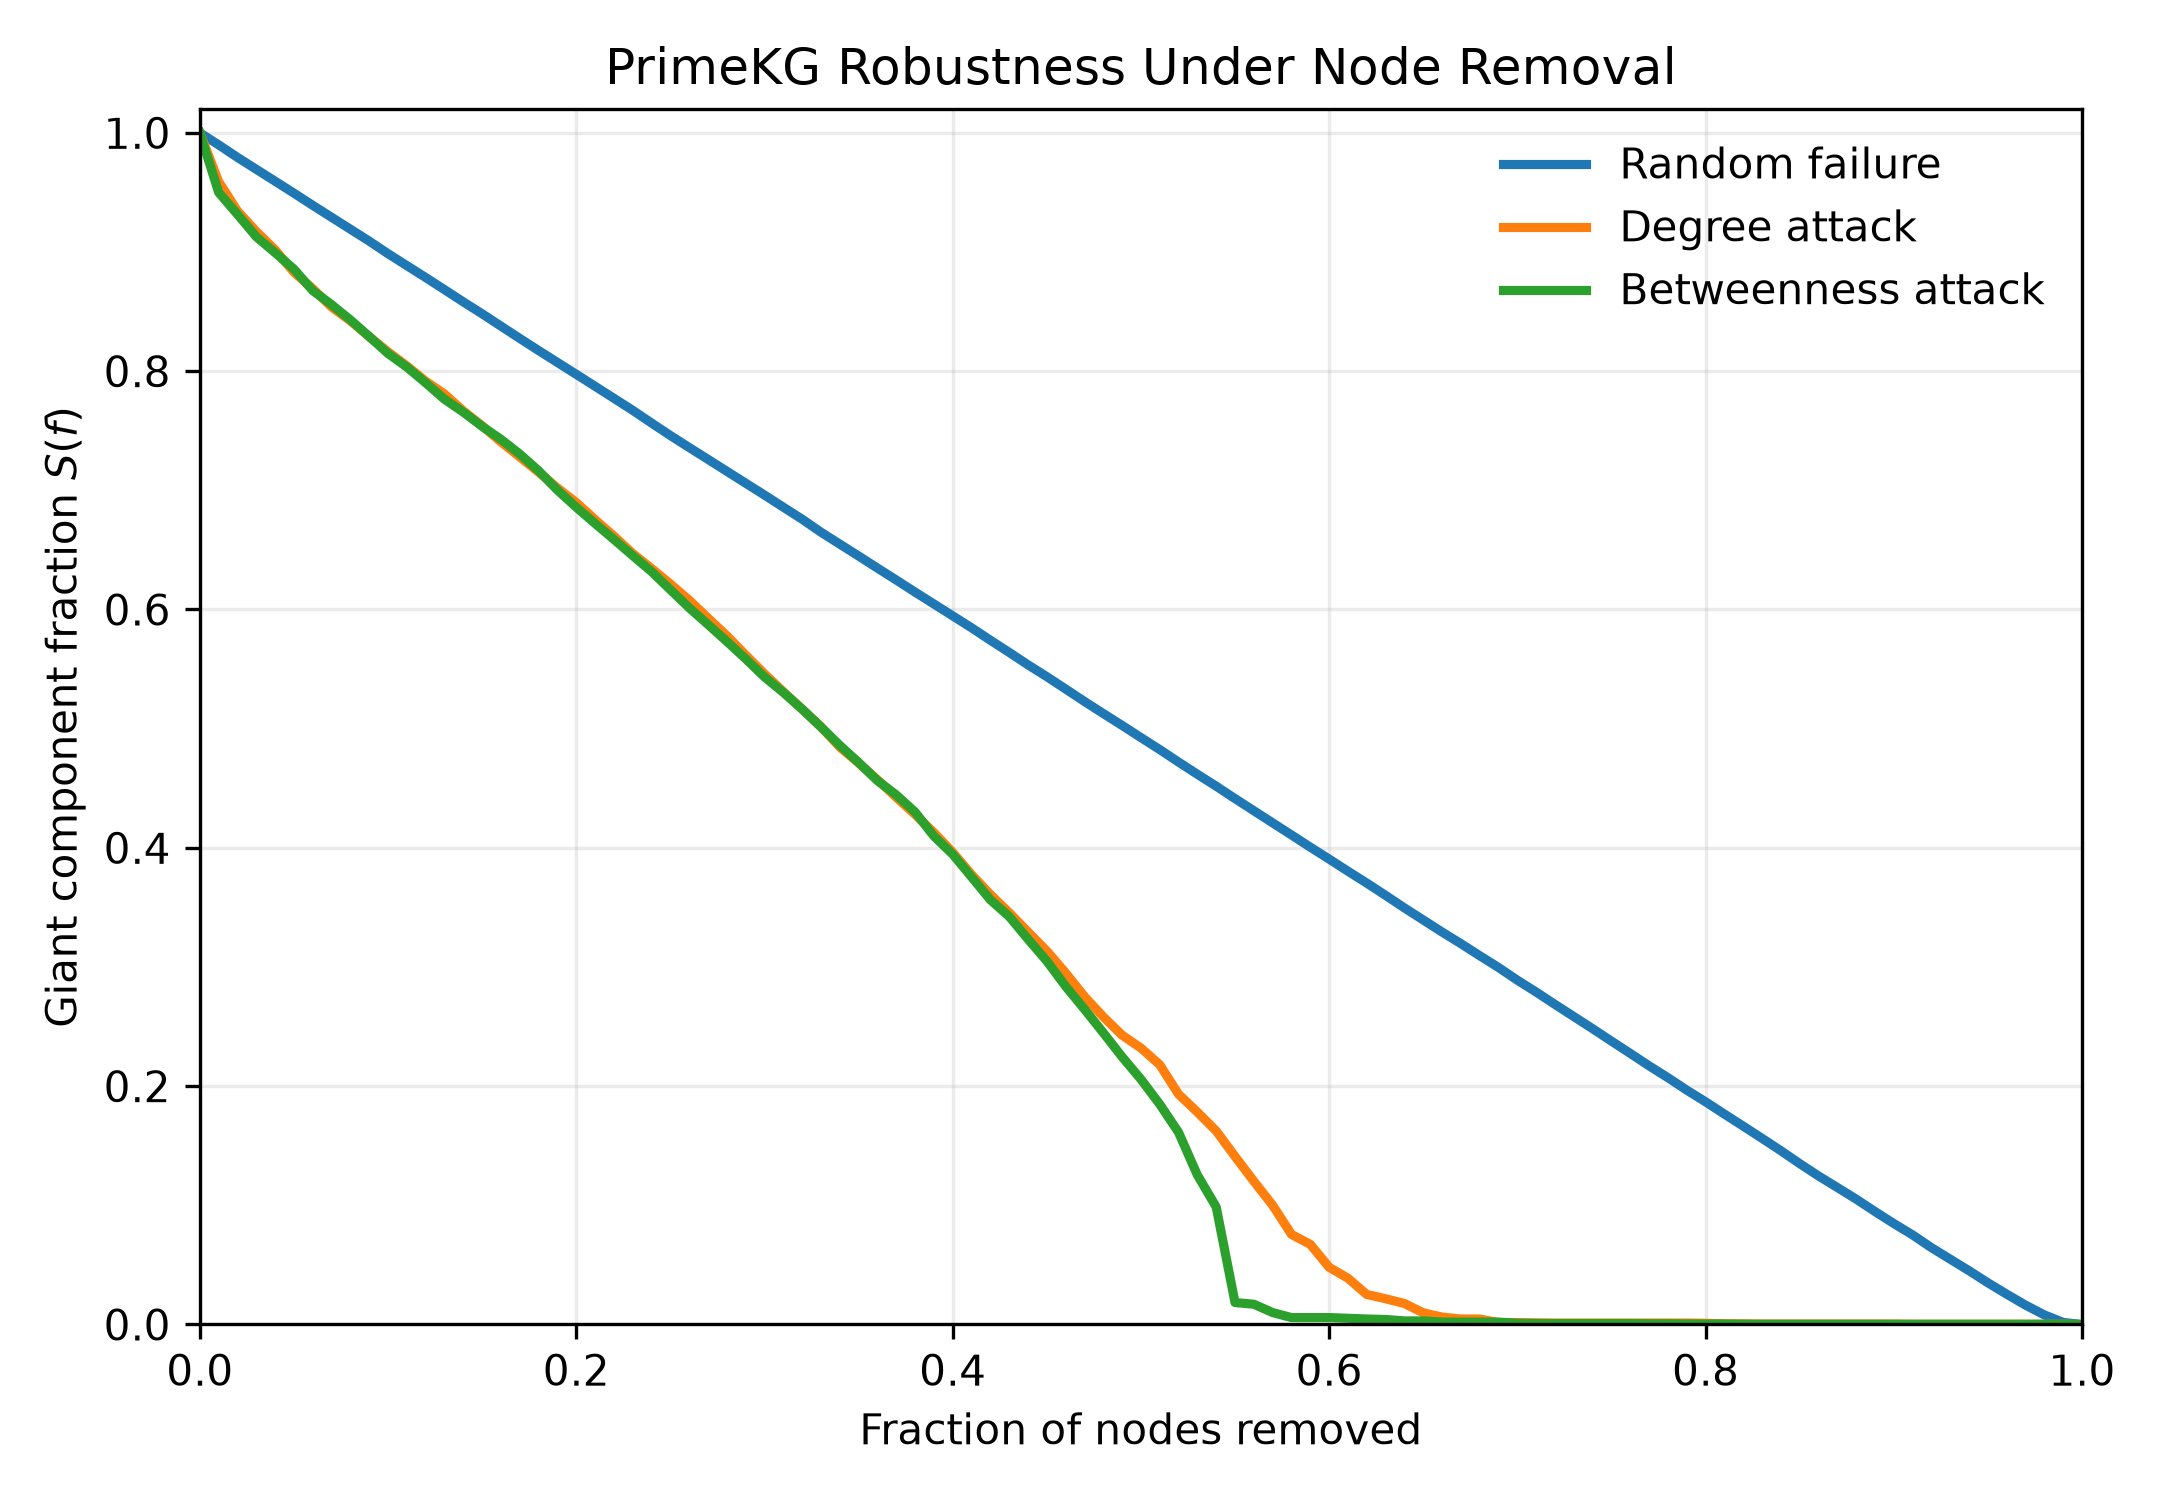
\includegraphics[width=0.86\linewidth]{ws2_attack_curves_primekg_5000_bfs_v1.png}%
    }{%
      \IfFileExists{figures/ws2_attack_curves_primekg_5000_bfs_v1.png}{%
        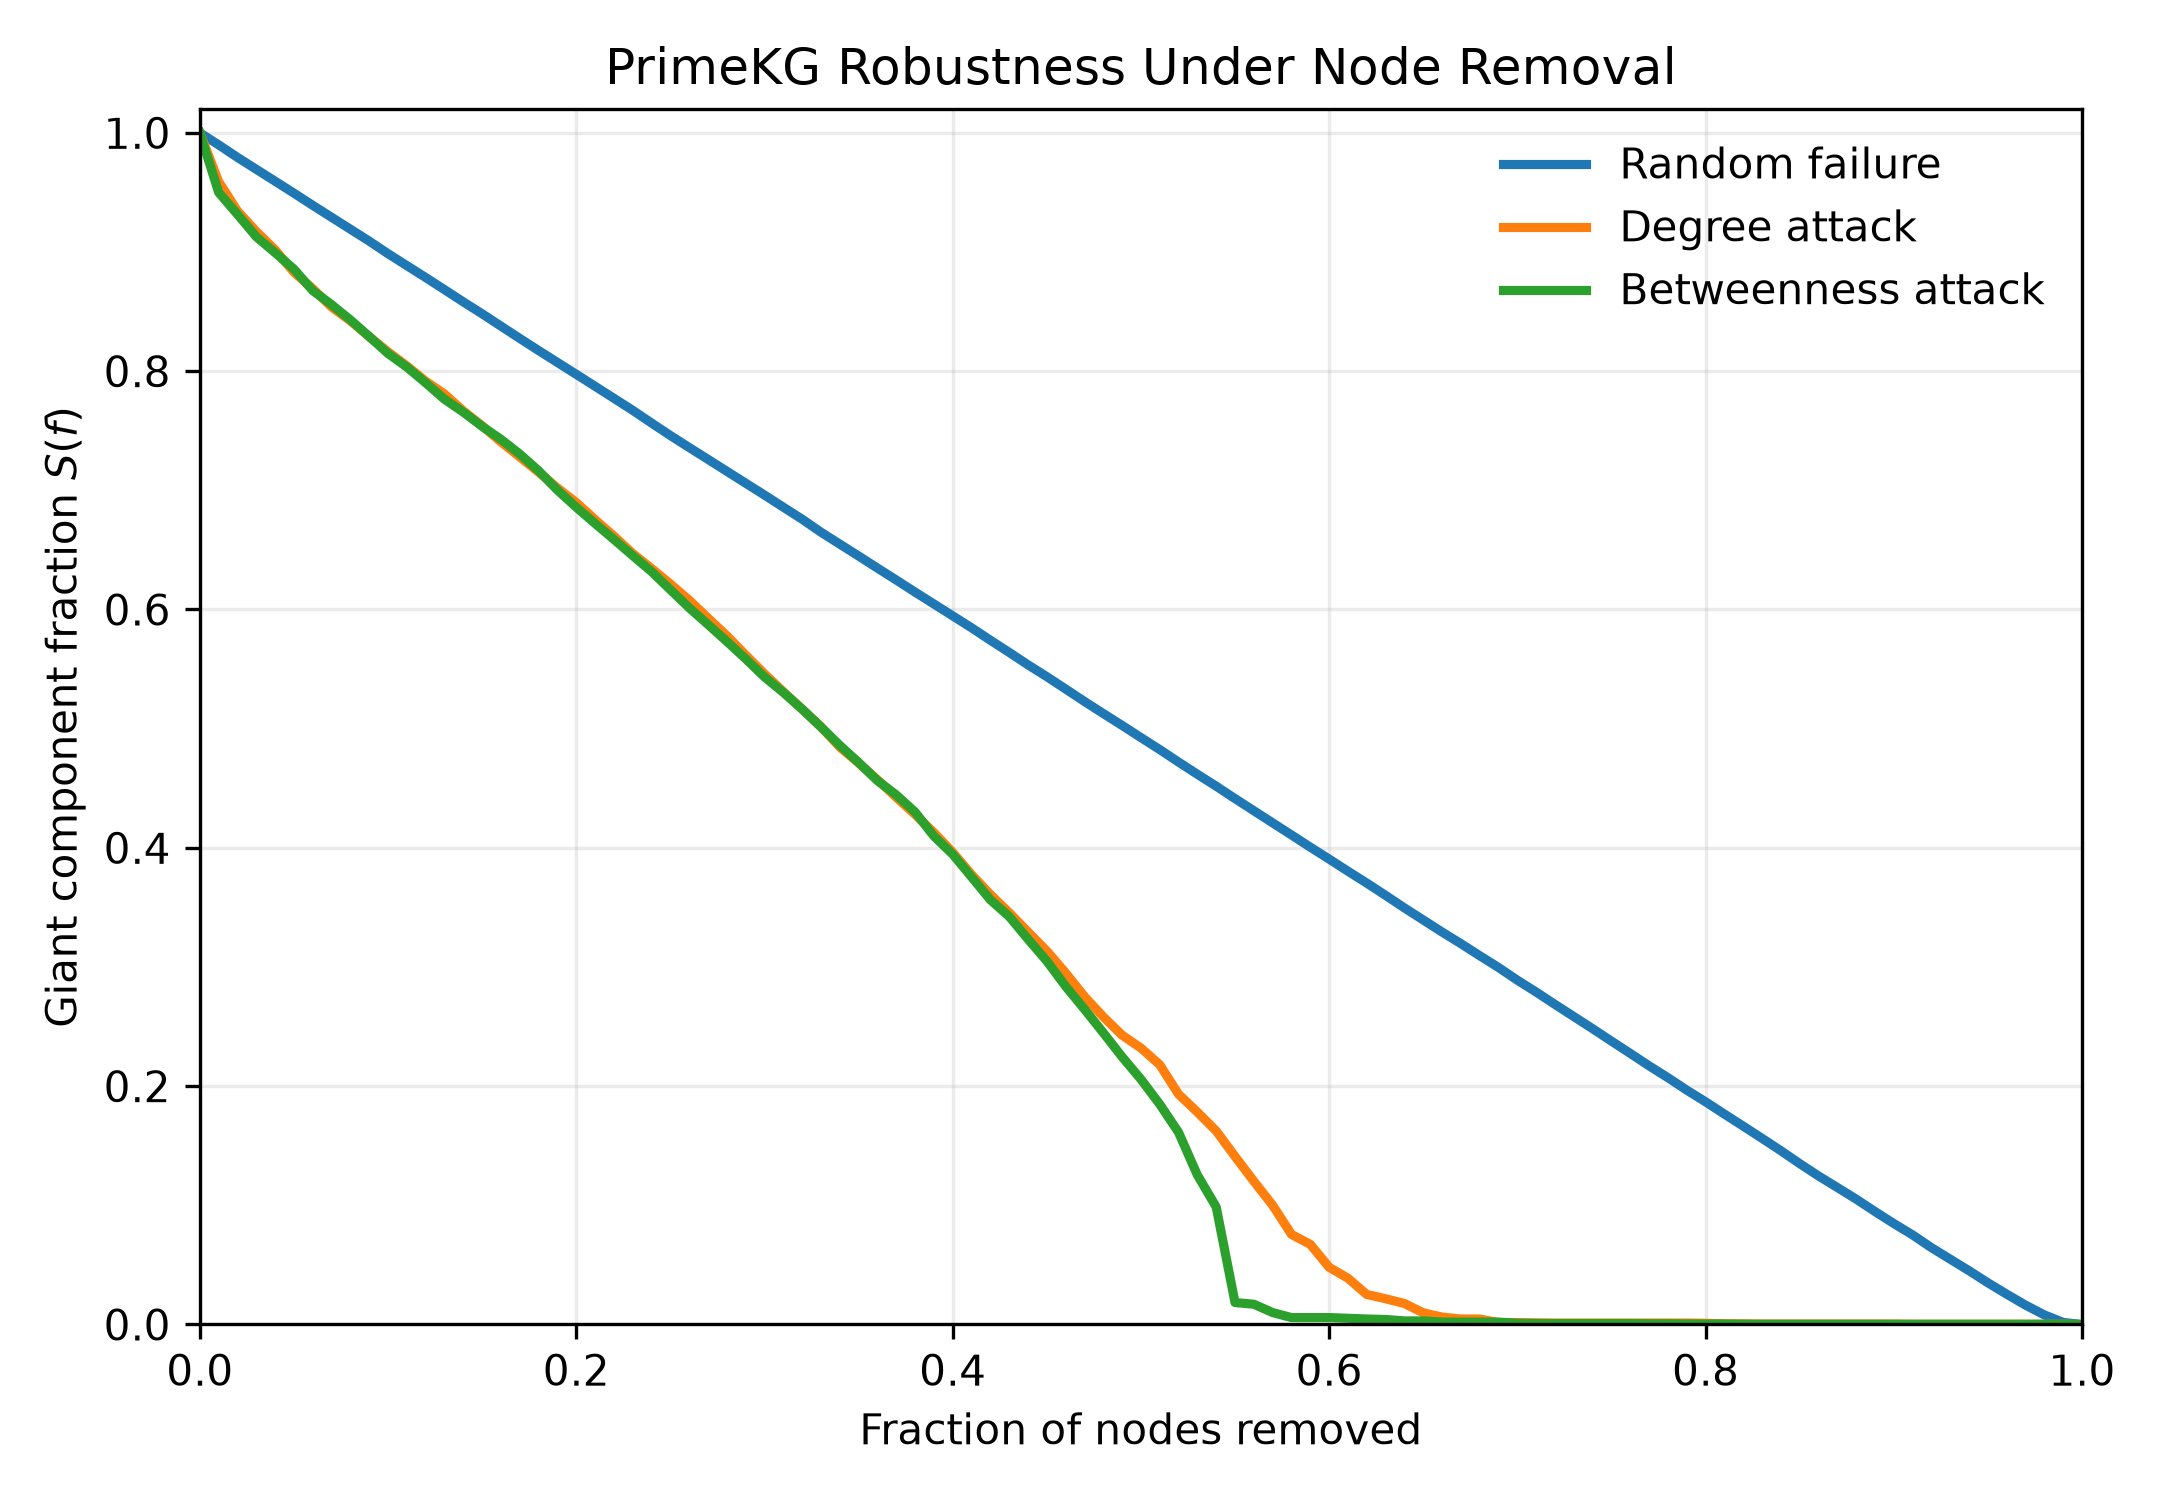
\includegraphics[width=0.86\linewidth]{ws2_attack_curves_primekg_5000_bfs_v1.png}%
      }{%
        \fbox{\parbox[c][2.2in][c]{0.82\linewidth}{\centering Placeholder: WS2 targeted-attack curve\\\texttt{figures/ws2\_attack\_curves\_primekg\_5000\_bfs\_v1.png}}}%
      }%
    }
    \caption{Structural robustness under random and targeted node removal. Degree and betweenness rankings are computed on the intact graph and kept fixed.}
    \label{fig:ws2-attacks}
\end{figure}

\begin{table}[H]
\centering
\caption{Selected GCC fractions under random and targeted node removal.}
\label{tab:ws2-gcc}
\begin{tabular}{@{}lccc@{}}
\toprule
Fraction removed & Random failure & Degree attack & Betweenness attack \\
\midrule
0.20 & 0.797 & 0.690 & 0.686 \\
0.50 & 0.493 & 0.232 & 0.206 \\
\bottomrule
\end{tabular}
\end{table}

These results show that robustness to random failure does not imply robustness to targeted failure. The PrimeKG subgraph is considerably more vulnerable when node removal is concentrated on structurally important entities. The similar behavior of the two targeted strategies also motivates examining whether the two centrality measures identify the same critical nodes.

\subsubsection{Composition and Overlap of Central Nodes}
The 5,000-node graph contains 4,643 gene/protein nodes, 283 disease nodes, and 74 drug nodes. Disease nodes therefore represent only $283/5000=5.66\%$ of the graph overall. However, within the top 1\% of the degree ranking, 16\% are disease nodes; within the top 1\% of the betweenness ranking, 14\% are disease nodes. Disease entities are therefore over-represented among structurally central nodes relative to their overall frequency in the graph.

\begin{figure}[H]
    \centering
    \IfFileExists{../figures/ws2_degree_hub_composition_primekg_5000_bfs_v1.png}{%
      \begin{subfigure}{0.48\linewidth}
      \centering
      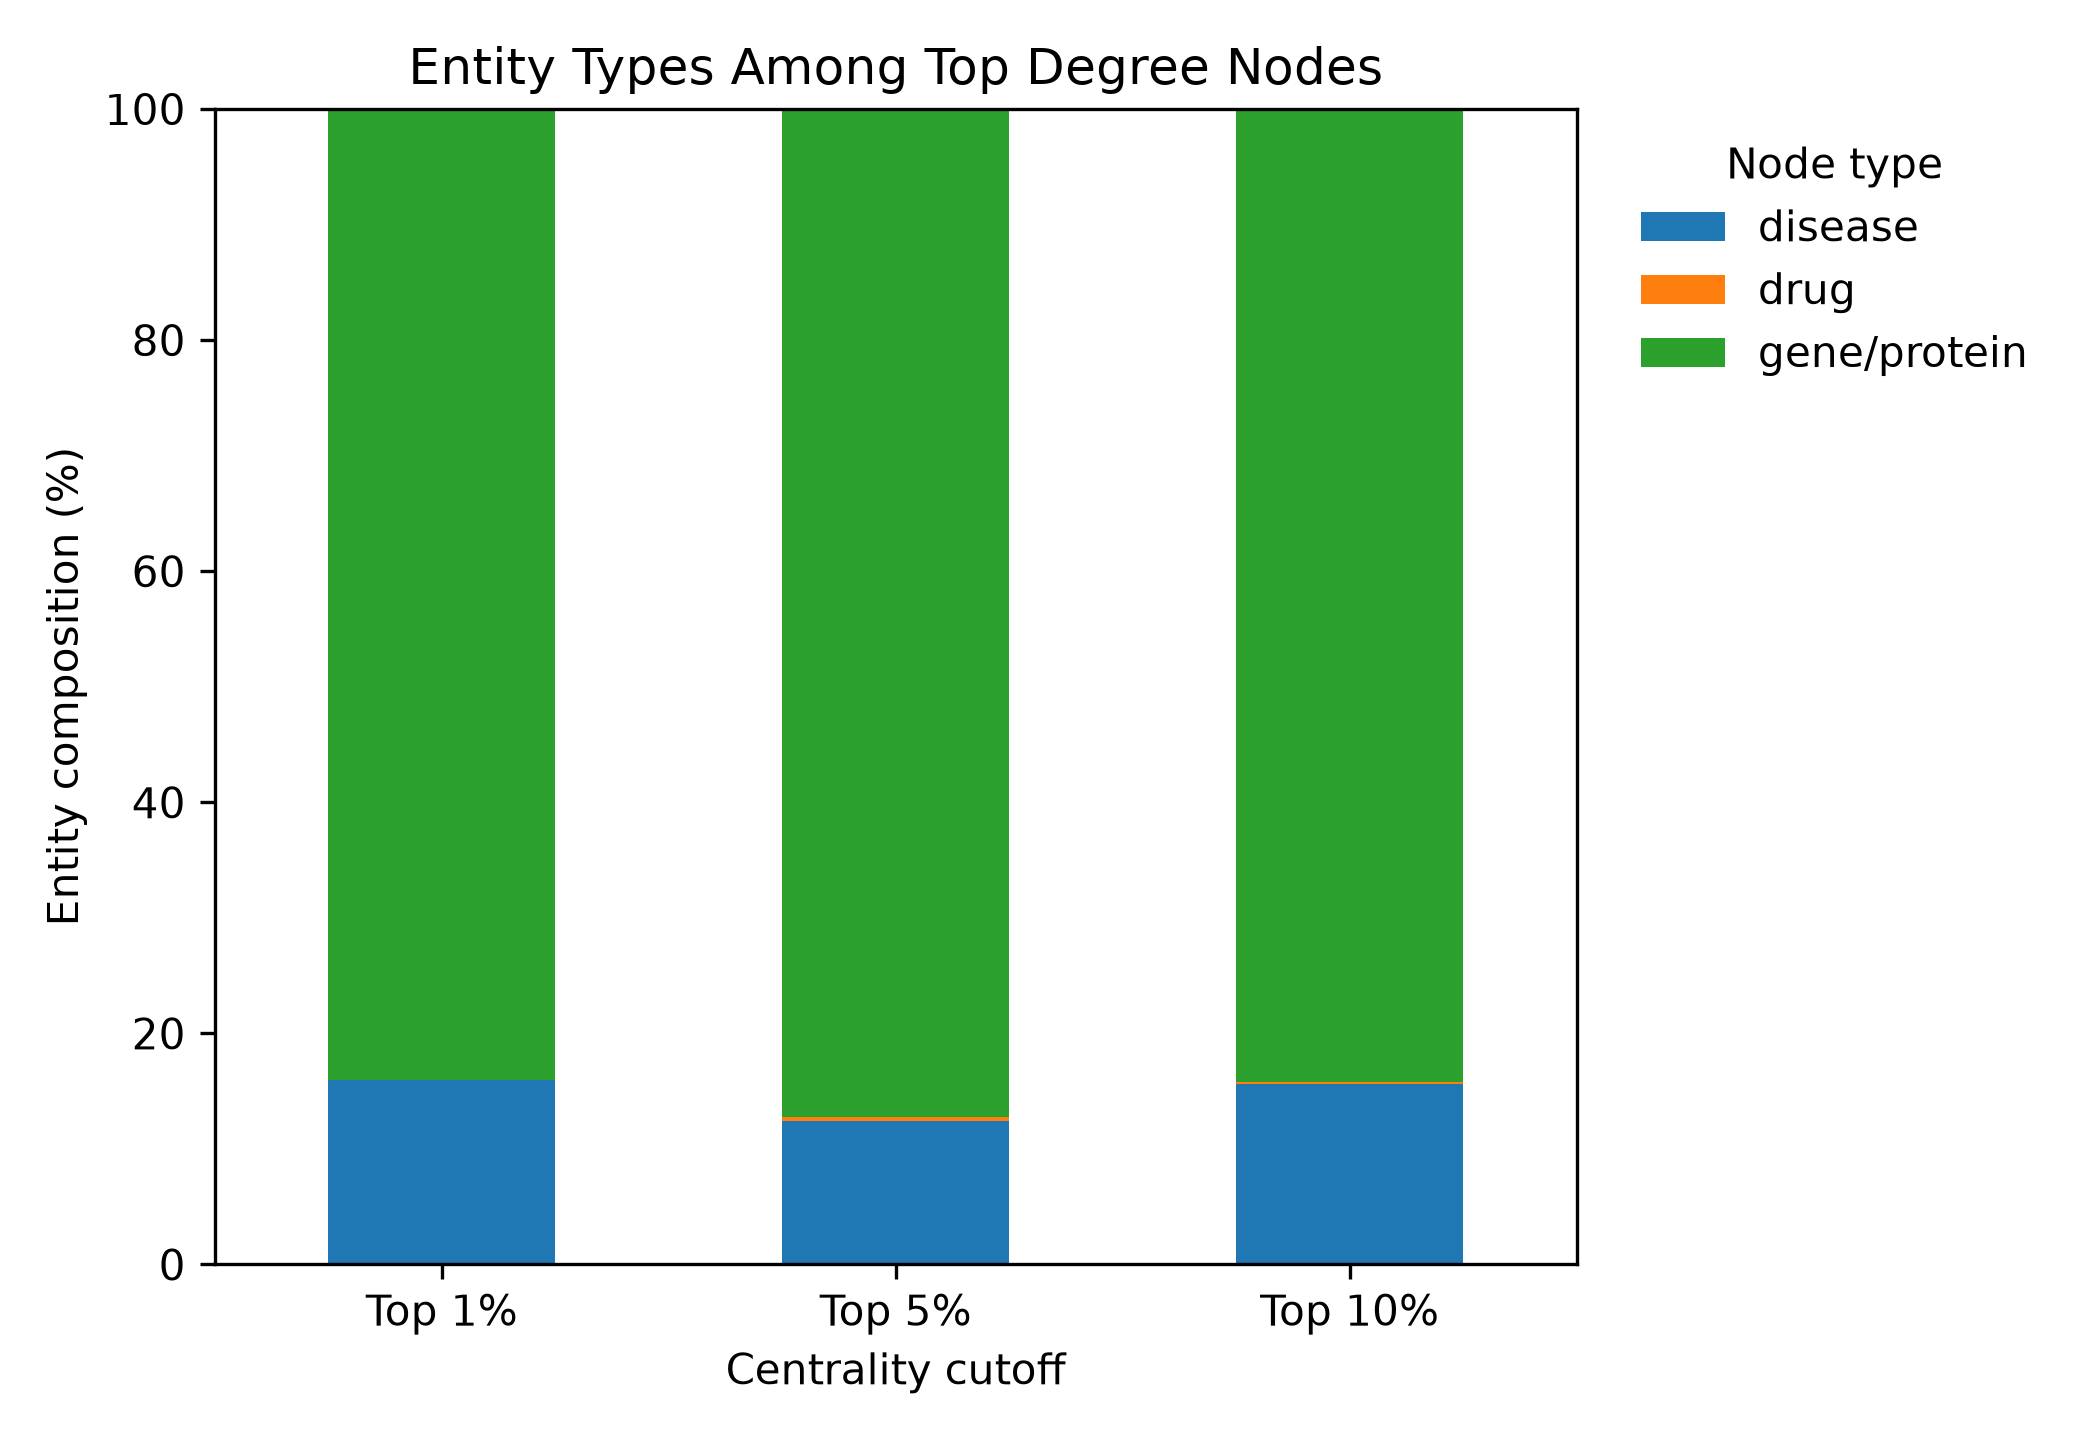
\includegraphics[width=\linewidth]{ws2_degree_hub_composition_primekg_5000_bfs_v1.png}
      \caption{Degree ranking}
      \end{subfigure}\hfill
      \begin{subfigure}{0.48\linewidth}
      \centering
      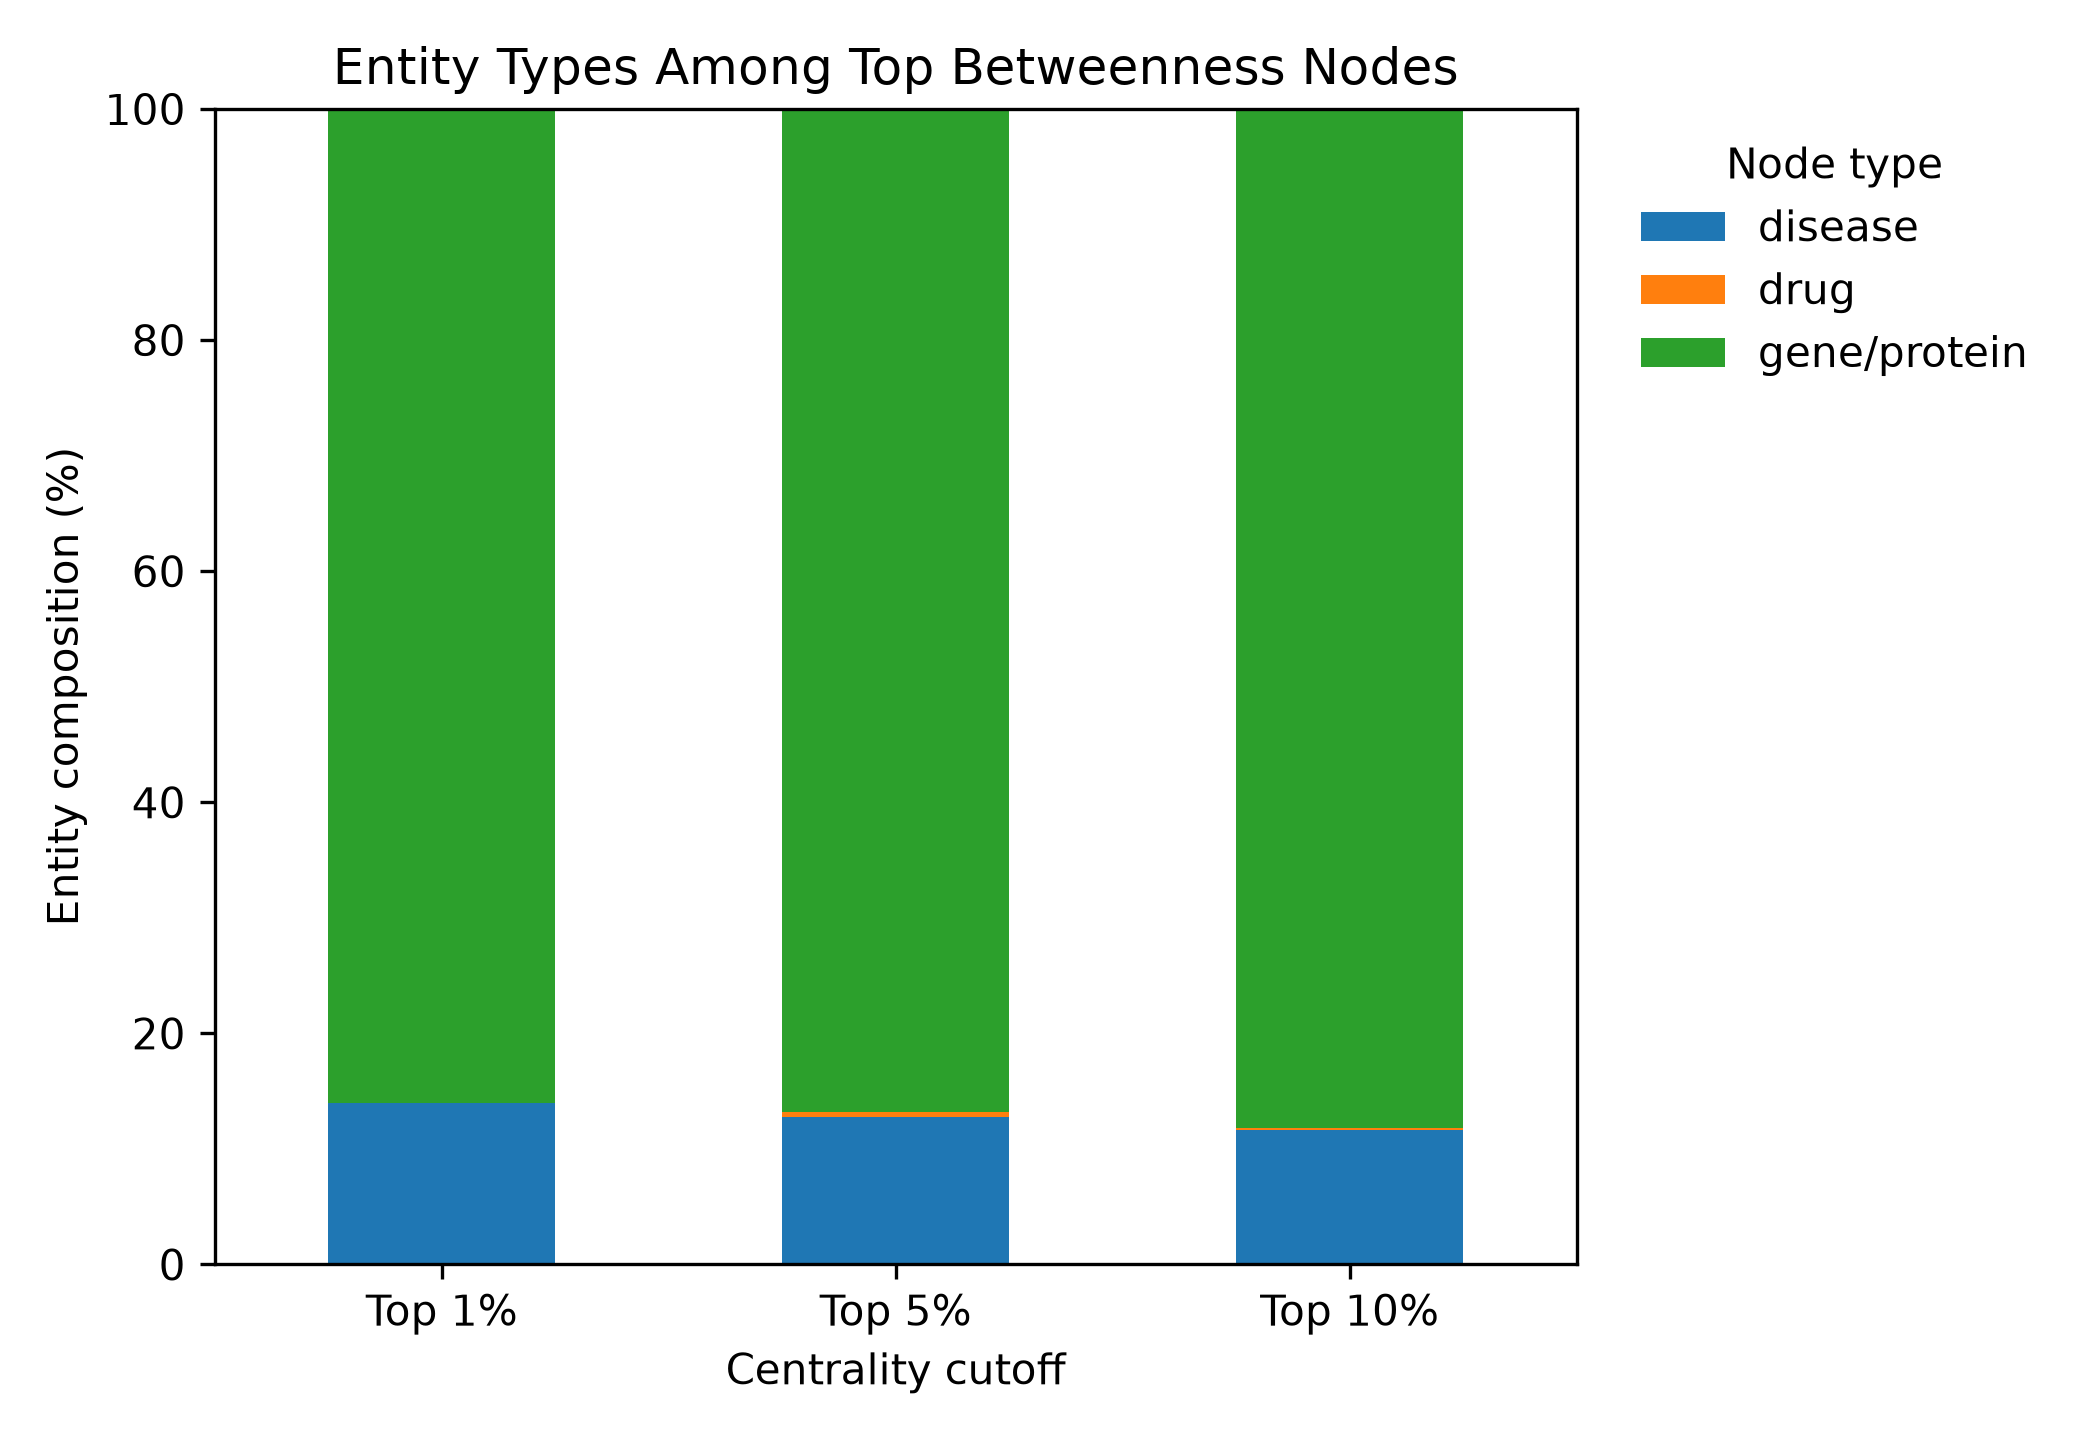
\includegraphics[width=\linewidth]{ws2_betweenness_hub_composition_primekg_5000_bfs_v1.png}
      \caption{Betweenness ranking}
      \end{subfigure}
    }{%
      \IfFileExists{figures/ws2_degree_hub_composition_primekg_5000_bfs_v1.png}{%
      \begin{subfigure}{0.48\linewidth}
      \centering
      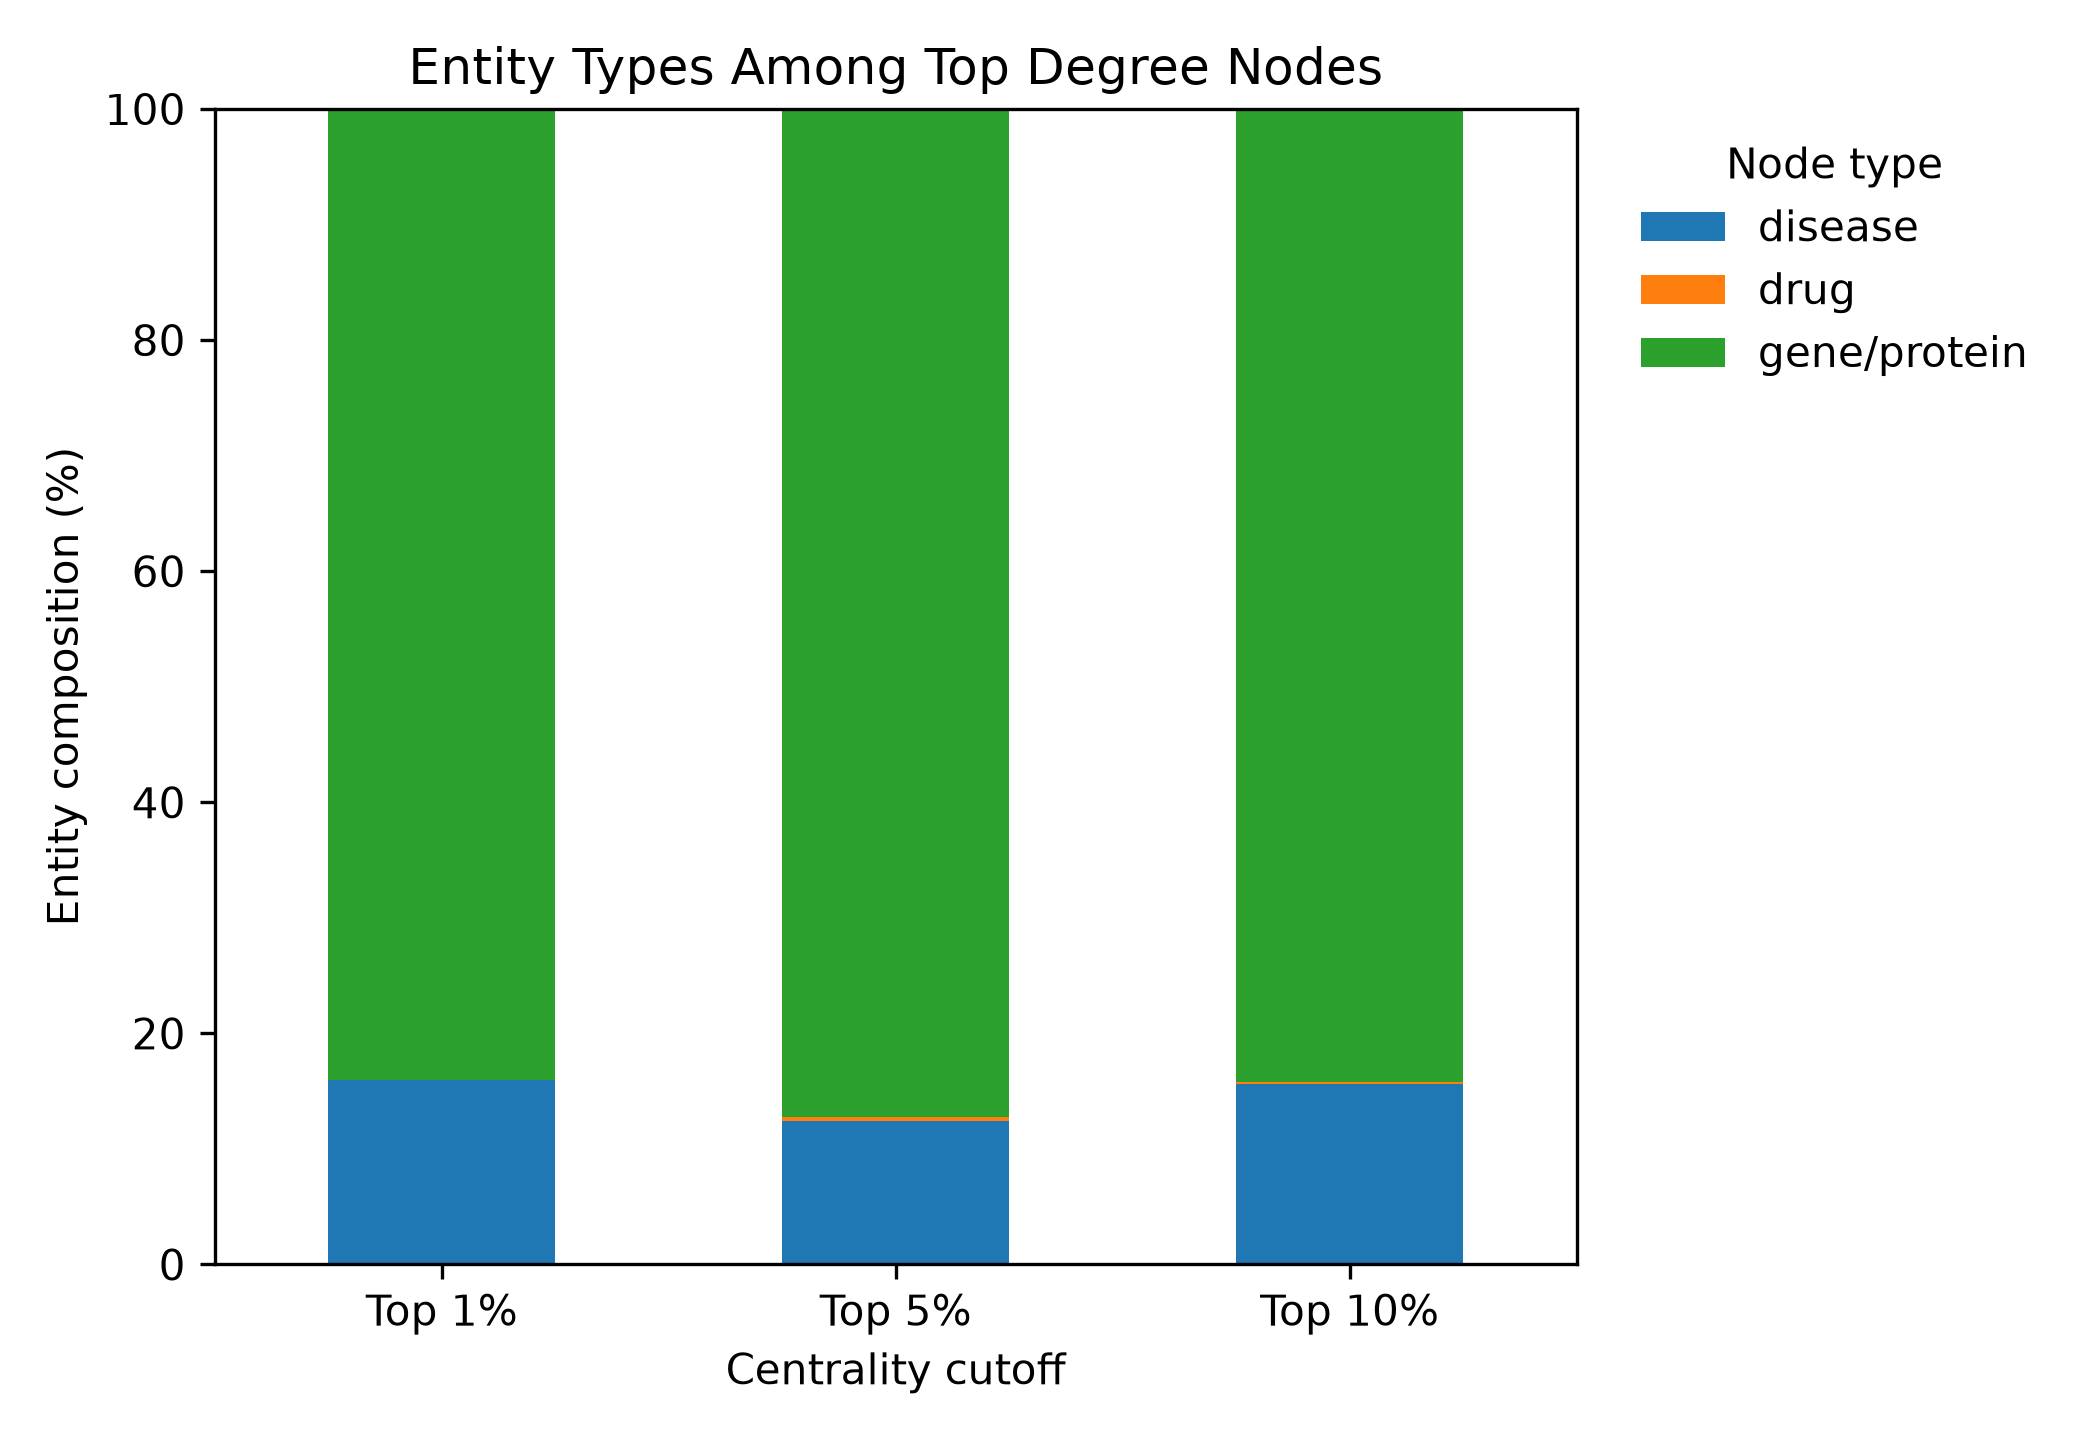
\includegraphics[width=\linewidth]{ws2_degree_hub_composition_primekg_5000_bfs_v1.png}
      \caption{Degree ranking}
      \end{subfigure}\hfill
      \begin{subfigure}{0.48\linewidth}
      \centering
      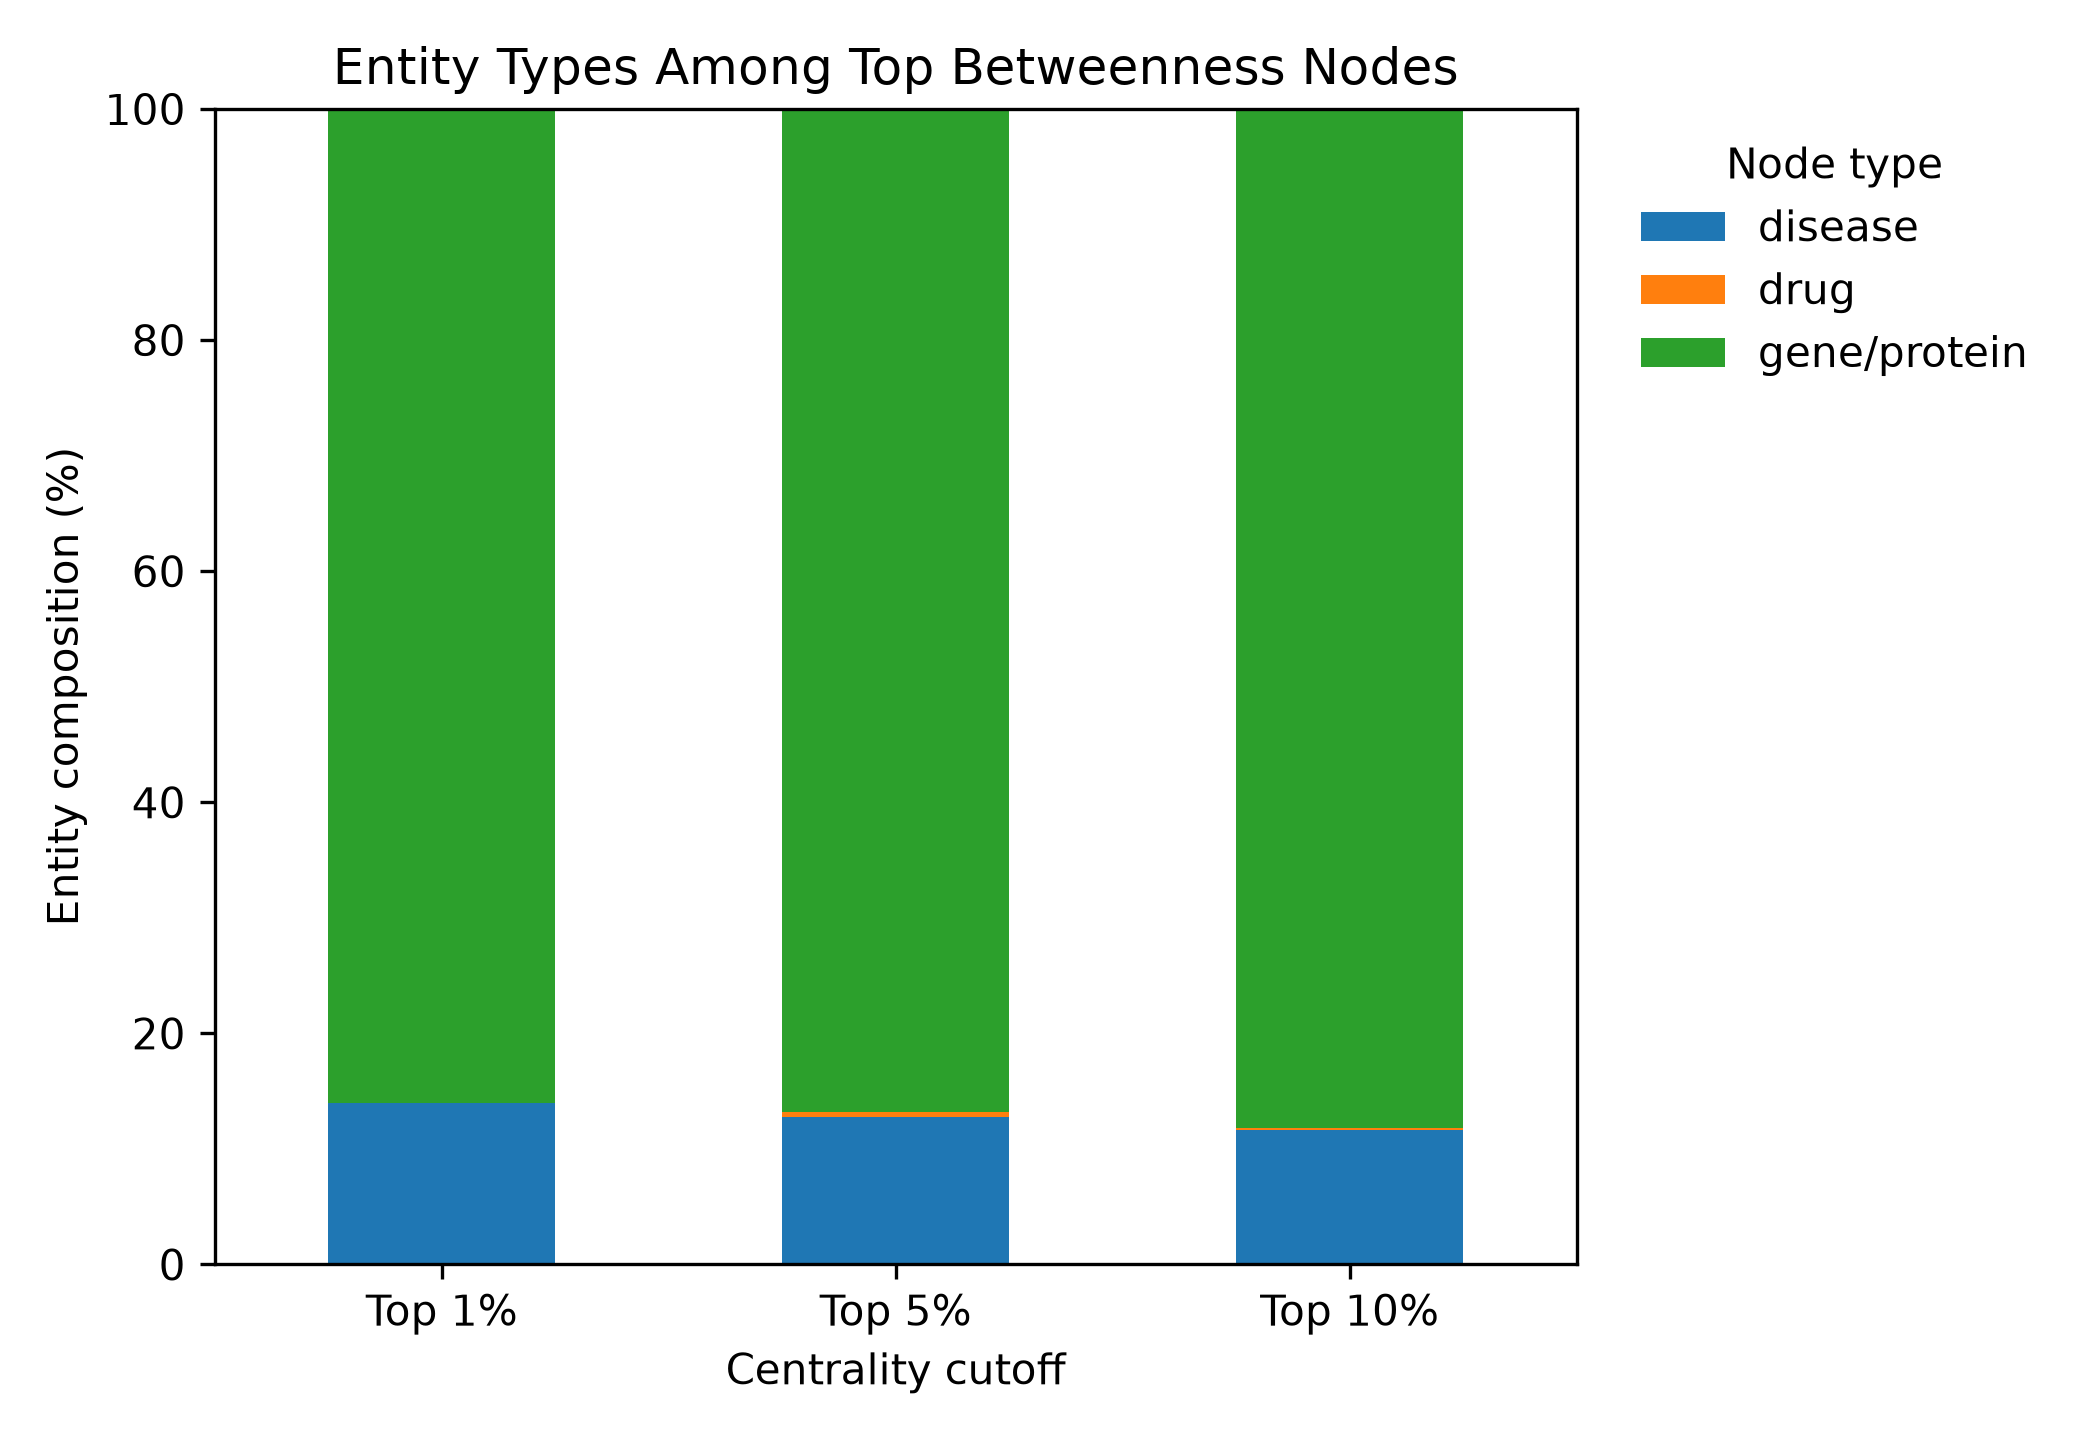
\includegraphics[width=\linewidth]{ws2_betweenness_hub_composition_primekg_5000_bfs_v1.png}
      \caption{Betweenness ranking}
      \end{subfigure}%
      }{%
      \fbox{\parbox[c][2.0in][c]{0.82\linewidth}{\centering Placeholder: central-node entity composition figures}}%
      }%
    }
    \caption{Entity-type composition among highly central nodes. Disease nodes constitute 5.66\% of the full graph but 14--16\% of the top 1\% central nodes.}
    \label{fig:ws2-composition}
\end{figure}

The two rankings also show substantial agreement at the individual-node level. Let $D_{50}$ and $B_{50}$ denote the top 50 nodes under degree and betweenness. Their intersection contains 41 nodes, and their Jaccard similarity is
\begin{equation}
J(D_{50},B_{50})=\frac{|D_{50}\cap B_{50}|}{|D_{50}\cup B_{50}|}=\frac{41}{59}\approx0.695.
\end{equation}
This strong overlap helps explain why the degree- and betweenness-based attack curves are similar: many nodes removed early under one ranking are also removed early under the other. The disease enrichment should be interpreted as a structural observation about this graph construction rather than as a direct biomedical claim.

\subsubsection{Comparison with the Theoretical Reference}
The final presentation also compares the empirical degree attack with the degree-based theoretical reference developed in Section~\ref{sec:theory}. The theoretical curve captures the broad collapse pattern but does not perfectly reproduce the empirical trajectory. This suggests that degree information alone does not capture every structural feature that influences the response of the empirical PrimeKG subgraph to targeted removal. The theoretical derivation and a systematic analysis of this discrepancy are left to the theory and prediction sections; here the comparison provides an empirical bridge between targeted robustness and the project's null-model analysis.

Overall, the targeted-attack experiments show that the identity of failed nodes matters strongly for structural robustness. Random node loss leaves a substantially larger connected core than removal of high-centrality nodes, while degree and betweenness identify a strongly overlapping critical set. The next section moves from structural robustness to functional robustness and asks whether drug--disease queries remain answerable after graph damage.
